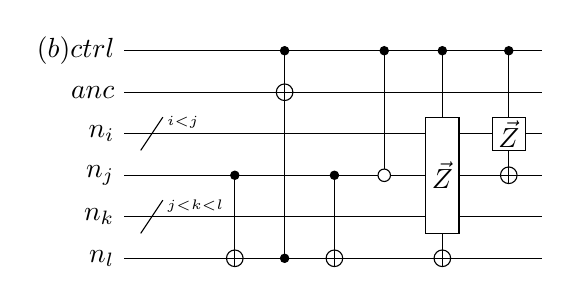
\begin{tikzpicture}[scale=1.000000,x=1pt,y=1pt]
\filldraw[color=white] (0.000000, -7.500000) rectangle (151.000000, 82.500000);
% Drawing wires
% Line 1: c W \text{(b) }ctrl
\draw[color=black] (0.000000,75.000000) -- (151.000000,75.000000);
\draw[color=black] (0.000000,75.000000) node[left] {$\text{(b) }ctrl$};
% Line 2: a W anc
\draw[color=black] (0.000000,60.000000) -- (151.000000,60.000000);
\draw[color=black] (0.000000,60.000000) node[left] {$anc$};
% Line 3: i W n_i
\draw[color=black] (0.000000,45.000000) -- (151.000000,45.000000);
\draw[color=black] (0.000000,45.000000) node[left] {$n_i$};
% Line 4: j W n_j
\draw[color=black] (0.000000,30.000000) -- (151.000000,30.000000);
\draw[color=black] (0.000000,30.000000) node[left] {$n_j$};
% Line 5: k W n_k
\draw[color=black] (0.000000,15.000000) -- (151.000000,15.000000);
\draw[color=black] (0.000000,15.000000) node[left] {$n_k$};
% Line 6: l W n_l
\draw[color=black] (0.000000,0.000000) -- (151.000000,0.000000);
\draw[color=black] (0.000000,0.000000) node[left] {$n_l$};
% Done with wires; drawing gates
% Line 8: i / ^{i<j}
\draw (6.000000, 39.000000) -- (14.000000, 51.000000);
\draw (12.000000, 48.000000) node[right] {$\scriptstyle{^{i<j}}$};
% Line 9: k / ^{j<k<l}
\draw (6.000000, 9.000000) -- (14.000000, 21.000000);
\draw (12.000000, 18.000000) node[right] {$\scriptstyle{^{j<k<l}}$};
% Line 10: c a i j k l LABEL width=-1
% Line 11: j +l
\draw (40.000000,30.000000) -- (40.000000,0.000000);
\filldraw (40.000000, 30.000000) circle(1.500000pt);
\begin{scope}
\draw[fill=white] (40.000000, 0.000000) circle(3.000000pt);
\clip (40.000000, 0.000000) circle(3.000000pt);
\draw (37.000000, 0.000000) -- (43.000000, 0.000000);
\draw (40.000000, -3.000000) -- (40.000000, 3.000000);
\end{scope}
% Line 12: c l +a
\draw (58.000000,75.000000) -- (58.000000,0.000000);
\filldraw (58.000000, 75.000000) circle(1.500000pt);
\filldraw (58.000000, 0.000000) circle(1.500000pt);
\begin{scope}
\draw[fill=white] (58.000000, 60.000000) circle(3.000000pt);
\clip (58.000000, 60.000000) circle(3.000000pt);
\draw (55.000000, 60.000000) -- (61.000000, 60.000000);
\draw (58.000000, 57.000000) -- (58.000000, 63.000000);
\end{scope}
% Line 13: j +l
\draw (76.000000,30.000000) -- (76.000000,0.000000);
\filldraw (76.000000, 30.000000) circle(1.500000pt);
\begin{scope}
\draw[fill=white] (76.000000, 0.000000) circle(3.000000pt);
\clip (76.000000, 0.000000) circle(3.000000pt);
\draw (73.000000, 0.000000) -- (79.000000, 0.000000);
\draw (76.000000, -3.000000) -- (76.000000, 3.000000);
\end{scope}
% Line 14: c -j
\draw (94.000000,75.000000) -- (94.000000,30.000000);
\filldraw (94.000000, 75.000000) circle(1.500000pt);
\draw[fill=white] (94.000000, 30.000000) circle(2.250000pt);
% Line 16: i j k G $\vec{Z}$ c +l
\draw (115.000000,75.000000) -- (115.000000,0.000000);
\begin{scope}
\draw[fill=white] (115.000000, 30.000000) +(-45.000000:8.485281pt and 29.698485pt) -- +(45.000000:8.485281pt and 29.698485pt) -- +(135.000000:8.485281pt and 29.698485pt) -- +(225.000000:8.485281pt and 29.698485pt) -- cycle;
\clip (115.000000, 30.000000) +(-45.000000:8.485281pt and 29.698485pt) -- +(45.000000:8.485281pt and 29.698485pt) -- +(135.000000:8.485281pt and 29.698485pt) -- +(225.000000:8.485281pt and 29.698485pt) -- cycle;
\draw (115.000000, 30.000000) node {$\vec{Z}$};
\end{scope}
\filldraw (115.000000, 75.000000) circle(1.500000pt);
\begin{scope}
\draw[fill=white] (115.000000, 0.000000) circle(3.000000pt);
\clip (115.000000, 0.000000) circle(3.000000pt);
\draw (112.000000, 0.000000) -- (118.000000, 0.000000);
\draw (115.000000, -3.000000) -- (115.000000, 3.000000);
\end{scope}
% Line 17: i G $\vec{Z}$ c +j
\draw (139.000000,75.000000) -- (139.000000,30.000000);
\begin{scope}
\draw[fill=white] (139.000000, 45.000000) +(-45.000000:8.485281pt and 8.485281pt) -- +(45.000000:8.485281pt and 8.485281pt) -- +(135.000000:8.485281pt and 8.485281pt) -- +(225.000000:8.485281pt and 8.485281pt) -- cycle;
\clip (139.000000, 45.000000) +(-45.000000:8.485281pt and 8.485281pt) -- +(45.000000:8.485281pt and 8.485281pt) -- +(135.000000:8.485281pt and 8.485281pt) -- +(225.000000:8.485281pt and 8.485281pt) -- cycle;
\draw (139.000000, 45.000000) node {$\vec{Z}$};
\end{scope}
\filldraw (139.000000, 75.000000) circle(1.500000pt);
\begin{scope}
\draw[fill=white] (139.000000, 30.000000) circle(3.000000pt);
\clip (139.000000, 30.000000) circle(3.000000pt);
\draw (136.000000, 30.000000) -- (142.000000, 30.000000);
\draw (139.000000, 27.000000) -- (139.000000, 33.000000);
\end{scope}
% Done with gates; drawing ending labels
% Done with ending labels; drawing cut lines and comments
% Done with comments
\end{tikzpicture}
